
\section{Flow control}
\index{flow control}
This section of the manual will describe how Angort handles conditional
code and loops. There are also several idioms using anonymous functions
which can be used for flow control, which will be described briefly.

\subsection{Conditions}
\index{conditions}
\label{conditions}
\indw{if}
\indw{then}
\indw{else}
These have the form:
\begin{v}
<condition> if <runs if true> then
\end{v}
The word \texttt{if} pops the item off the top of the stack,
and jumps forward to just after the corresponding \texttt{then} if it is false (zero).
There is also a two way branch:
\begin{v}
<condition> if <runs if true> else <runs if false> then
\end{v}
This works the same way, except that the \texttt{if} jumps to after the
\texttt{else} if the top value is false, and \texttt{else} jumps forward
to just after \texttt{then}. This is shown in the figure below:
\begin{center}
\includegraphics[width=5in]{ifthen.pdf}
\end{center}
Here is a code example, printing whether a number is even or odd:
\begin{lstlisting}
:evenodd 
    # Get the number on the stack modulo 2, and use
    # whether it is zero or not as the condition.
    2 % if
        "number is odd"     # stack this string if there is a remainder
    else
        "number is even"    # stack this string if remainder is zero
    then                    # end the conditional
    .                       # print the top of the stack
;
\end{lstlisting}
We can run this with various values:
\begin{v}
1|0> 4 evenodd
number is even
1|0> 3 evenodd
number is odd
\end{v}
Conditions can be nested.


\subsection{Multi-line flow control and ``slugs''}
\index{slugs}
\label{multilineflow}
It is important to note that Angort processes input on a line-by-line
basis when not defining a function, both within a script and in immediate
mode. Therefore, code like the following will not work:
\begin{lstlisting}
read len 0 = if
    "zero length string"
then
\end{lstlisting}
while the following will:
\begin{lstlisting}
read len 0 = if "zero length string" then
\end{lstlisting}
With the former code, Angort will attempt to compile and run the first line,
and will find that the line has no matching \texttt{then}. This will not
occur on the latter example because the \texttt{then} is provided on
the same line. This will not happen while a function is being defined,
because Angort suspends compilation until the function is completed
with a semicolon.

While this is a limitation when writing scripts it is easily surmounted
by either putting code into a named function, or defining and immediately
running an anonymous function. Anonymous functions are enclosed with 
parentheses, leaving the function on the stack. They can then be run
with \texttt{call} or \texttt{@} (the two are equivalent). Thus
the above can be written
\begin{lstlisting}
(
    read len 0 = if
        "zero length string"
    then
)@
\end{lstlisting}
In informal conversations I have taken to referring to anonymous
functions which are called immediately as ``slugs,'' both from
the typesetting terminology and from the visual appearance
of \texttt{(....)@}.


\subsection{Case blocks}
\indw{case}
\indw{otherwise}
\indw{cases}
In order to avoid testing if..else..then constructions where a number of
different, mutually exclusive cases need to be tested, the ``case block''
structure is provided, which emulates the ``elsif'' construction in other
languages.

Case blocks begin with \texttt{cases}, and each case consists
of 
\begin{v}
    <condition> if <action> case
\end{v}
The case block must end, after the final case, with
\begin{v}
    <default action> otherwise
\end{v}
An example:
\begin{lstlisting}
:test |a:|
    cases
        ?a 0 = if "It's Zero". case
        ?a 1 = if "It's One". case
        ?a 2 = if "It's Two". case
        ?a 3 = if "It's Three". case
        ?a 4 = if "It's Four". case
        ?a 5 = if "It's Five". case
        ?a 6 = if "It's Six". case
        ?a 7 = if "It's Seven". case
        "It's something else".   otherwise
    
;
\end{lstlisting}
This function will print an appropriate message for integers from 0 to 7,
and ``It's something else'' for any other value.

\subsection{Loops}
\label{loops}
\index{loop}
\indw{each}
\def\opencurlybrace{\{}
\def\closecurlybrace{\{}
\indw{\opencurlybrace}
\indw{\closecurlybrace}
\indw{leave}\indw{ifleave}
There are two kinds of loops in Angort --- infinite loops,
which must be broken out of using \texttt{leave} or \texttt{ifleave}; and
iterator loops, which loop over a collection (i.e. a hash or list) or
a range. Both are delimited with curly brackets \verb+{}+, but iterator loops
use the \texttt{each} word before the opening brace.

\subsubsection{Infinite loops}
\index{loop!infinite}
Any \texttt{leave} word will break out of an infinite loop:
\begin{lstlisting}
( |:counter|         # a local variable "counter", no parameters
    0 !counter          # set counter to zero
    {                   # start loop
        ?counter.       # print the counter
        !+counter       # increment the counter
        ?counter 100=   # is it equal to 100?
        if leave then   # if so, leave the loop
    }
)@
\end{lstlisting}
This will count from 0 to 99. Note the use of an anonymous function
as described in Section~\ref{multilineflow}, which contains a local
variable \texttt{counter}.
The sequence
\begin{lstlisting}
if leave then
\end{lstlisting}
is so common that it is coded to a special word of its own, and can be written
as 
\begin{lstlisting}
ifleave
\end{lstlisting}
The function above could be written tersely as
\begin{lstlisting}
(|:c| 0!c {?c. !+c ?c 100= ifleave)@;
\end{lstlisting}
This is still using a slug (see Sec.~\ref{multilineflow})
because we require the local variable
provided by the anonymous function.
Loops can be nested, and the \texttt{leave} words will jump out of the
innermost loop in which they appear.

\subsubsection{Iterator loops}
\indw{i}\index{loop!iterator}
Iterator loops loop over an \emph{iterable} value. These typically currently ranges,
hashes and lists, but ints and longs are also iterable (see below). They are delimited by curly braces like infinite loops,
but are preceded by the 
\texttt{each} word. This pops the iterable off the stack and makes an
iterator out of it, over which the loop runs. The iterator exists for as 
long as the loop does, and is destroyed when the loop completes. Again, iterator
loops can be nested (and can be nested with infinite loops). If we use
an iterator loop to iterate over a range object,
the counting example can be rewritten as:
\begin{lstlisting}
(
    0 100 range         # stack a range from 0-99 (see below)
    each {              # start the iterator loop
        i               # push the current item in the iterator
        .               # print it
    }                   # end of loop
)@
\end{lstlisting}
Here, the \texttt{range} word takes two integers $a,b$ from the stack which define
an integer range $\{x\in \mathbb{Z} \mid a \le x < b\}$.
Note that range end value is exclusive --- that is, it is the first value which
is \emph{not} in the range --- so the above example, specified as
\texttt{0 100 range}, actually counts from 0 to 99. 
This looks somewhat odd with integer ranges, but serves to prevent float ranges
relying on equality tests:
\begin{lstlisting}
(
    0 10 0.09 frange    # float range from 0-10 in steps of 0.09
    each {i.}           # print them
)@
\end{lstlisting}
will print about 9.990008 as its final value. Because this doesn't require
any local variables, it works as an immediate mode one-liner:
\begin{lstlisting}
0 10 0.09 frange {each i.}
\end{lstlisting}

Although we've not covered lists and hashes yet, it's useful to know that we can
iterate over the values in a list. For example
\begin{lstlisting}
[1,2,3,4,5] each {i.}
\end{lstlisting}
will print the numbers from 1 to 5. Similarly, we can iterate over the keys 
and values of a hash:
\begin{lstlisting}
[% "foo" "bar", "baz" "qux"] each {i.}
\end{lstlisting}
will print the hash's keys: ``foo'' and ``bar'', while
\begin{lstlisting}
[% "foo" "bar", "baz" "qux"] each {i p "=" p ival.}
\end{lstlisting}
\indw{ival}
will print ``key=value'' for each entry. Here, \texttt{ival} gets the value
(as opposed to the key)
of the current pair in the iterator, 
and \texttt{p} prints without a newline.

\subsubsection{Iterating ints and longs}
Ints and longs are also iterable, which might seem a little odd,
but acts as a handy shorthand. If you create an iterator over a positive int
or long $n$, it will count up from 0 to $n-1$. If it's negative, it will
count down from 0 to $n+1$. This means instead of doing this to run
a piece of code 10 times:
\begin{lstlisting}
0 10 range each {...}
\end{lstlisting}
you can do this:
\begin{lstlisting}
10 each {...}
\end{lstlisting}
Inside the loop the value of both \texttt{i} and \texttt{iidx} is the
current iterator value; \texttt{iidx} has no value and will be an error
(cannot get value of item in non-collection).



\subsubsection{Nested iterator loops}
\label{nestit}
Each loop has its own iterator, even if they come from the same iterable:
\begin{lstlisting}
( |:r|
    0 10 range !r           # store a range
    ?r each {               # outer loop
        i.                  # print value of outer loop iterator
        ?r each {           # inner loop
            i.              # print value of inner loop iterator
        }
    }
)@
\end{lstlisting}
The range here is used twice, generating two separate iterators with
their own current value.

\indw{j}\indw{k}
While the word \texttt{i} retrieves the iterator value inside the current
loop, inside nested iterator loops it is often useful to get the value
in outer loops. This can be done with the \texttt{j} and \texttt{k} words,
to get the outer and next outer iterator values:
\begin{lstlisting}
( |:r|
    0 10 range !r           # store a range
    ?r each {               # outer loop
        ?r each {           # inner loop
            i j +           # print sum of inner and outer iterators
        }
    }
)@  
\end{lstlisting}
\indw{jval}\indw{kval}
The \texttt{jval} and \texttt{kval}
words also exist to get a hash iterator value for two outer iterator loops.

\clearpage  
\subsection{The state of the stack inside a loop}
Note that the iterator is not kept on the normal stack --- it is popped
off when the loop starts and kept inside a special stack. The same
applies to infinite loops: no loop state is kept on the stack. This 
leaves the stack free for manipulation:
\begin{lstlisting}
# sum all the integers from 0 to x inclusive    
:sumto |x:|
    0               # stack an accumulator
    0 ?x 1+ range   # stack a range from 0 to x inclusive
    each {          # stack an iterator, then pop it onto the iterator stack
        i           # get current iterator value
        +           # add it to the accumulator
    }               # end loop
;                   # finish and return the accumulator
\end{lstlisting}
Note that this isn't actually how you'd do it: \texttt{reduce} is
more efficient:
\begin{lstlisting}
:sumto |x:| 0 0 ?x 1+ range (+) reduce;
\end{lstlisting}
This more functional style of programming is dealt with in
Section~\ref{functional}.

\subsection{Words to create ranges}
\indw{range|textbf}\indw{frange|textbf}\indw{srange|textbf}
There are three words to create a range on the stack:
\begin{center}
\begin{tabular}{|l|l|p{4in}|}\hline
\textbf{name} & \textbf{stack picture} & \textbf{side-effects and notes}\\ \hline
range & (x y -- range) & create an integer range over the interval $[x,y)$ with a step of 1; i.e. a range from $x$ to $y-1$ inclusive.\\
srange & (x y s -- range) &  create an integer range over the interval $[x,y)$ with a step of $s$\\
frange & (x y s -- range) &  create an float range over the interval $[x,y)$ with a step of $s$\\
\hline
\end{tabular}
\end{center}
See Section~\ref{stackpic} for how stack pictures define the parameters
and return values for a function.

\subsection{Explicit iterators}
\indw{mkiter}\indw{icur}\indw{inext}\indw{idone}\indw{ifirst}
It's sometimes necessary to use iterators manually instead of creating
them automatically with "each" and getting the values using "i" in an
iterator loop.
To do this, we have the following words:
\begin{center}
\begin{tabular}{|l|l|p{4in}|}\hline
\textbf{name} & \textbf{stack picture} & \textbf{side-effects and notes}\\ \hline
mkiter & (iterable -- iterator) & create an iterator\\
icur & (iterable -- item) & get the current item\\
inext & (iterable --) & advance the iterator\\
idone & (iterable -- bool) & return 1 if the iterator is at the last item\\
ifirst & (iterable --) & reset the iterator to the start\\
iter & (-- iterable) & return the iterator which is being iterated over in
the current loop\\
\hline
\end{tabular}
\end{center}


You might need this when you want to iterate over
two collections in parallel, for example in implementing the \texttt{zipWith}
function\footnote{\texttt{zipWith} is already built into Angort,
this is just an illustrative example.}. This function takes two collections, and runs a binary function on
pairs of items, each from one of the collections, returning a list:

\begin{v}
    ["foo","bar"] ["fish","zing"] (+) zipWith each{i.}
\end{v}
\noindent would print
\begin{v}
    foofish
    barzing
\end{v}
This could be implemented by using an index to go over both lists:

\begin{lstlisting}
    :zipWith |a,b,f:|
        [] # stack an empty list
        0 ?a len ?b len min range each {
            i ?a get # get from first list
            i ?b get # get from second list
            ?f call # call the function
            , # and append to the list
        }
;
\end{lstlisting}
but a more elegant solution might be:
\begin{lstlisting}
    :zipWith |a,b,f:it|
        ?b mkiter !it
        []
        ?a each {
            ?it idone ifleave # exit if explicit iterator done
            i # get loop iterator value
            ?it icur # get explicit iterator value
            ?f@, # call the function and append to the list
            ?it inext # advance the explicit iterator
        }
    ;
\end{lstlisting}
Here, we use an each loop to iterate over list a, and an explicit
iterator to iterate over list b.

\subsection{Conditional compilation}
The normal \textbf{if..else..then} construction doesn't help
if you want a piece of code to be completely ignored by Angort,
for example when it refers to a library that may not be loaded.
In that case, you don't want Angort to try to compile the code
at all because it won't be able to resolve the identifiers to
the unloaded library. Consider the code
\begin{lstlisting}
0!Threads
(
    ?Threads if
        `thread library drop
        0 mythreadfunction thread$create !Thread
    then
)@
\end{lstlisting}
This will fail because the thread library won't load, but Angort
still needs to compile the \texttt{thread\$create} call.

To fix problems like this, the \textbf{compileif} directive can skip entire
lines. Because it reads the value on the stack top it is compiled as an
opcode, so don't put it inside a function and make sure it ends the line it's
on. The skipping stops when the \textbf{endcompileif} directive is found on a
line by itself. The above code could then be rewritten
\begin{lstlisting}
0!Threads
?Threads compileif
    `thread library drop
    0 mythreadfunction thread$create !Thread
endcompileif
\end{lstlisting}
There is also the \textbf{elsecompileif} directive, which works as
you would expect:
\begin{lstlisting}
0!Threads
?Threads compileif
    `thread library drop
    thread$mutex !MyMutex
    0 mythreadfunction thread$create !Thread
    :lock ?MyMutex thread$lock
    :unlock ?MyMutex thread$unlock
elsecompileif
    :lock ;
    :unlock ;
endcompileif
\end{lstlisting}
Note that \textbf{compileif clauses cannot be nested.} 
Those caveats in full:
\begin{itemize}
\item \textbf{compileif} structures cannot be nested;
\item \textbf{ifcompile} should end a line;
\item \textbf{elsecompileif} and \textbf{endcompileif} should be on
a line by themselves;
\item \textbf{compileif}, \textbf{elsecompileif} and \textbf{endcompileif} cannot
be inside a function definition (anonymous or otherwise).
\end{itemize}

